\chapter{Implementation}\label{C:implementation}


\section{PWM Signal Generation}\label{S:pwm_gen_impl}

The PWM signal generator subsystem was designed around the Espressif ESP32 microcontroller. For ease of development around this microcontroller, a pre-built breadboard compatible development board was purchased for the implementation. \\

Using this development board, a PWM hardware driver was developed to facilitate the implementation of this subsystems core functionality as specified in \Cref{S:specs_design}. This driver implements three core functions, `\lstinline{PWM_setup()}' to initialise the PWM hardware, `\lstinline{PWM_set_duty()}' to select a new duty cycle, and `\lstinline{PWM_set_frequency}' to select a new frequency. The full driver implementation can be found in \Cref{A:pwm_code}.\\

After the software implementation had been completed, it was identified that the 3.3V digital output of the microcontroller would be incapable of driving the buck converters switching power MOSFET. To resolve this, the IR2125 high side N-channel gate driver IC was purchased to drive the MOSFET from the PWM generators output signal. This final circuit was then implemented and it's functionality was tested on a breadboard. Please see \Cref{A:pcb_and_schematic} for the designed schematic, and \Cref{A:breadboard} for the implemented breadboard circuit.

% Discuss how the micro will be unable to directly drive the gate of the switching MOSFET, as it's $V_{GS_{on}}$ will be too large. Because of this a gate driver will need to be selected. The driver will need to be driven using the 3.3V logic from the ESP32, and will need timings fast enough to function correctly at 100kHz. I can also discuss how during the lock-down I was unable to purchase a gate driver, and so I built a bootstrapping circuit from components I located around the house. 


\section{System State Sensing}\label{S:current_sense_impl}

% Due to time restraints caused by COVID-19 related delays, the implementation and evaluation of each design within the state sensing subsystem discussed in \Cref{S:sensing_design} was impractical. Therefore, designs that \todo{lacked prior formal testing and evaluation in the form of datasheets} were prioritised for implementation. 

\subsection{Output Voltage Sensing}\label{S:v_sense_impl}

The output voltage sensing design discussed in \Cref{S:v_sense_design} was implemented on a prototyping breadboard. Please see \Cref{A:pcb_and_schematic} for the designed schematic, and \Cref{A:breadboard} for the implemented breadboard circuit.

Using the ESP32 development board, an ADC hardware driver was developed to facilitate the measurement of the sensor output. This driver implements the core functionality of the ADC though two functions, `\lstinline{init_adc()}' to assign the input IO and measurement resolution, and `\lstinline{read_adc()}' to take an ADC measurement. Using these two functions this driver then also facilitates the computation of a rolling average with the `\lstinline{rolling_average()}' function, and voltage conversion with the `\lstinline{adc_conversion()}' function. The full driver implementation can be found in \Cref{A:adc_code}.\\

When initially implementing the ADC conversion function, it was assumed that that the output conversion of the ADC was linear. Once this had been implemented, it was observed that there were large inaccuracies in the voltage conversion. 

From this it was identified that the internal ADC  was non-linear, and would require calibration before meeting the required specifications. To achieve this, ADC measurements were taken for a selection of known input voltages ranging from 100mV to 3V in 500mV steps. These ADC measurements were then plotted against their respective input voltages using Matlab, and a forth order polynomial was fit to the data, shown in \Cref{F:adc_calibration}. This polynomial was then used for the conversion of the raw ADC reading to a voltage, greatly improving the ADC's accuracy.

\begin{figure}[!h]
    \centering
    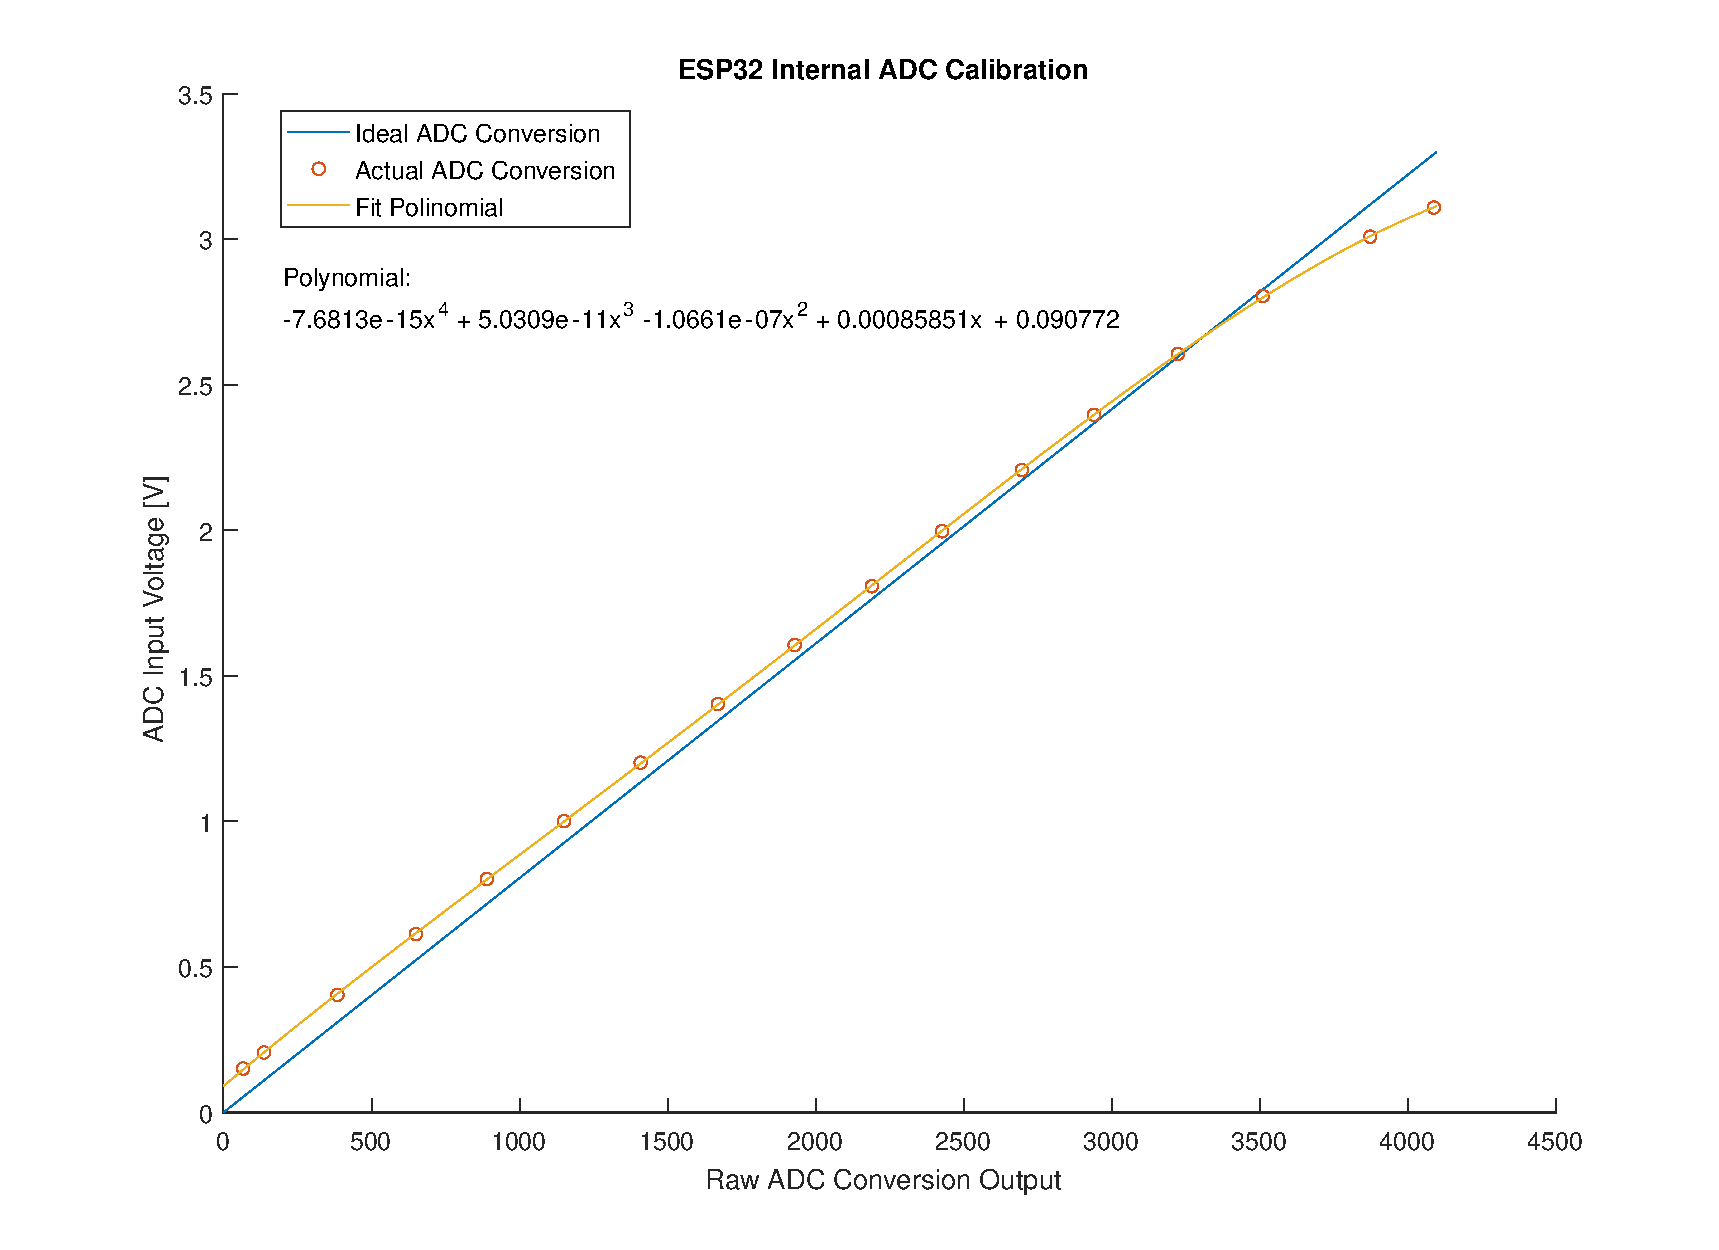
\includegraphics[width = 0.9\textwidth]{adc/calibration.pdf}
    \caption{ESP32 internal ADC calibration data with forth order polynomial fit}
    \label{F:adc_calibration}
\end{figure}

\subsection{Inductor Current Sensing}

\subsubsection*{Average Inductor Current Sensing}

The average inductor current sensing design discussed in \Cref{S:avg_current_design} was implemented on a prototyping breadboard. Please see \Cref{F:final_peak_detector} for the designed schematic, and \Cref{A:breadboard} for the implemented breadboard circuit.

This design also utilises the ESP32 internal ADC, which was previously implemented in \Cref{S:v_sense_impl}. Therefore no further implementation was required for the functionality of this design.  


\subsubsection*{Peak Inductor Current Sensing}

The peak inductor current sensing design discussed in \Cref{S:peak_current_design} was initially implemented on a prototyping breadboard, using an LT084CN operational amplifier (op amp) provided by the lab technicians. 

On implementation it was observed that the functional principles of the design held true, as the design maintained a DC output voltage that was dependant in the input peak to peak ripple. However it was observed that the accuracy of the design was much lower than expected when compared to the design simulations. The operation of this original design \todo{can be seen in} \Cref{A:peak_detector}.\\

It was identified that the limiting factor within the design was the bandwidth and slew-rate of the input stage op amp seen in \Cref{F:sample_and_hold_circuit}. This op amp is responsible for charging the sampling capacitor and negating the forward bias diode drop, and therefore it's bandwidth and slew-rate will dictate the bandwidth of the design.  

Based on this, the input op amp was replaced with the OPA2830, as it provided a greatly improved bandwidth of 230MHz and a slew rate of 500V/$\mu$s. The original design was also altered to place a potentiometer in series with the sampling capacitor, as well as adding a high impedance resistor in parallel with this capacitor. This allows for the final designs performance to be tuned through the potentiometer, and any overshoot to be quickly dissipated by the parallel discharge resistor. This final design of the schematic can be seen in \Cref{F:final_peak_detector}, and the implemented breadboard circuit can be found in \Cref{A:breadboard}.

\begin{figure}[!h]
    \centering
    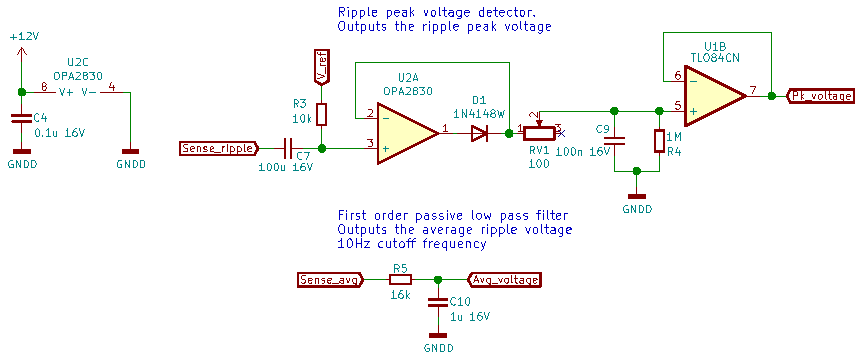
\includegraphics[width = 0.95\textwidth]{pcb/peak_detector_schematic.pdf}
    \caption{Finalised peak detector schematic, with updated op amp selection and performance improvements}
    \label{F:final_peak_detector}
\end{figure}


\section{Control System}\label{S:control_impl}

The control system design discussed in \Cref{S:control_design} has been implemented in the form of a generic PID based control system library. This control system implementation provides a structure in which all of the controller variables and states are stored. This simplifies the initialisation of the controller, as the proportional, integral, derivative, and time period constants can all be specified at the structure initialisation. This implementation also allows for the creation and management of multiple controllers simultaneously, meeting requirements 2 \& 4. 

This control library also provides more advanced safety features for the system, including selectable minimum and maximum output limits, and selectable integrator windup limits.\\

This library implements two core functions which provide the full functionality of a digital PID control loop. `\lstinline{PID_init()}' initialises and sets up the controller, and `\lstinline{PID_update()}' calculates the new output of the controller. The full driver implementation can be found in \Cref{A:pid_code}.


\section{Full system implementation}

\subsubsection*{Software implementation}

The full system software implementation is built upon the ESP-IDF framework, and utilises a FreeRTOS to provide tasks and scheduling. 

The ESP-IDF Framework was chosen over other supported frameworks due to it's increased control of the ESP32 available hardware peripherals, which was required for the designs system to meet it's specified requirements from \Cref{F:sys_overview}. 

The use of the ESP-IDF framework also facilitated the use of FreeRTOS, providing access to a task scheduler that would greatly decrease the structural complexity of this system. This scheduler allows each subsystem within the design to operate from within a task, independent of all others. therefore, this implementation reduces the complexity of further developments within this project, without limiting the functionality of the microcontroller platform. The full system software implementation can be found in \Cref{A:main_code}.


\subsubsection*{Hardware implementation}

To facilitate the ease of use of the fully designed system, a printed circuit board (PCB) was designed and implemented using the KiCAD software platform. This PCB implements all finalised designed elements discussed in \Cref{C:design}, and provides multiple footprints for the buck converter output filter to allow for expedited testing and varying filters. For the full system schematic, please refer to \Cref{A:pcb_and_schematic}.

\begin{figure}[!h]
    \centering
    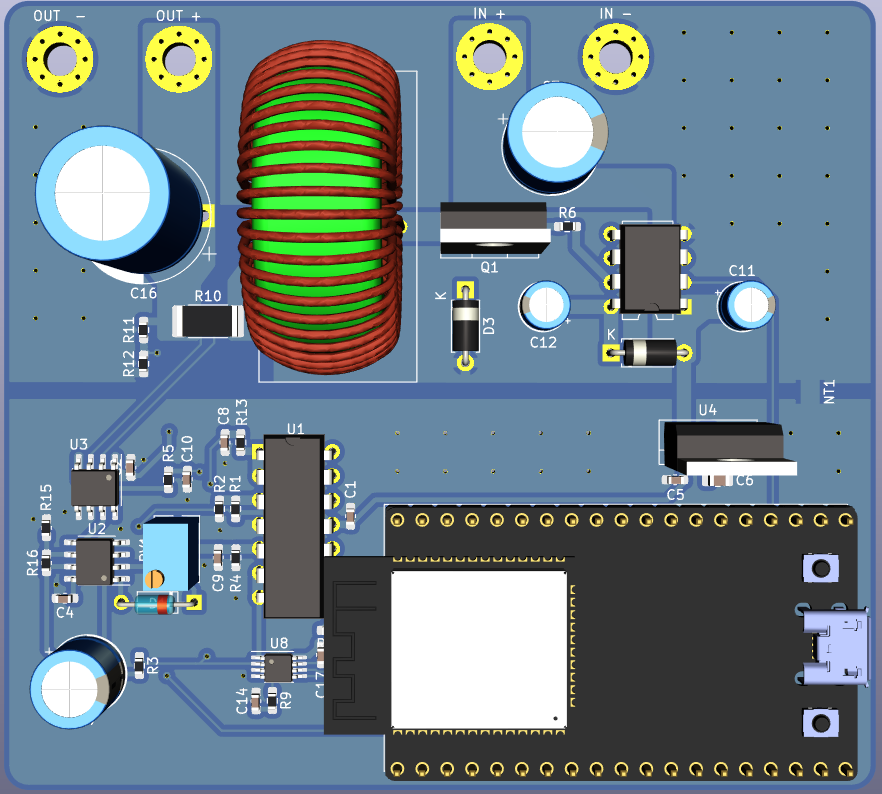
\includegraphics[width = 0.85\textwidth]{pcb/pcb_render.png}
    \caption{Full system printed circuit board implementation}
    \label{F:implemented_pcb}
\end{figure}

% Discuss how the code implements each of the hardware sections designed. Then also discuss how the full system has been implemented on a PCB 
% Discuss the ESP-IDF HAL (Hardware Abstraction Layer), and how it provides greater control of the system resources than the more commonly used Arduino platform. 
% \\
% Then discuss how the system operates within the freeRTOS real time operating system, what allows for easy multitasking between the different time sensitive control loops that will have to be run on the micro.  
% \\
% Finally discuss the simple to use API that was implemented, which aims to abstract away the HAL layer. This API is implemented using collection of single header libraries written in the 'C' programming language, with each implementing only the core functionality of the hardware they are interacting with. This makes the software platform robust and simple to move to different embedded platforms, with such a move only requiring the re-implementation of the core functions of each library. 